% Opcje klasy 'iithesis' opisane sa w komentarzach w pliku klasy. Za ich pomoca
% ustawia sie przede wszystkim jezyk oraz rodzaj (lic/inz/mgr) pracy.
\documentclass[shortabstract,inz]{iithesis}
\usepackage[utf8]{inputenc}
\usepackage{natbib}
\usepackage{graphicx}
\usepackage{subcaption}
\usepackage{float}
\usepackage[nottoc]{tocbibind}
\usepackage[obeyspaces]{url}
\usepackage{listings}
\usepackage[T1]{fontenc}
\usepackage{inconsolata}

\usepackage{color}

\definecolor{pblue}{rgb}{0.13,0.13,1}
\definecolor{pgreen}{rgb}{0,0.5,0}
\definecolor{pred}{rgb}{0.9,0,0}
\definecolor{pgrey}{rgb}{0.46,0.45,0.48}

\usepackage{listings}
\lstset{language=Java,
  showspaces=false,
  showtabs=false,
  breaklines=true,
  showstringspaces=false,
  breakatwhitespace=true,
  commentstyle=\color{pgreen},
  keywordstyle=\color{pblue},
  stringstyle=\color{pred},
  basicstyle=\ttfamily,
  moredelim=[il][\textcolor{pgrey}],
  moredelim=[is][\textcolor{pgrey}]{\%\%}{\%\%}
}


\polishtitle    {Koncepcja i implementacja systemu do zarządzania budżetem domowym}
\englishtitle   {Concept and implementation of home budget managment system}
\polishabstract {Celem pracy było stworzenie koncepcji i implementacja systemu służącego do zarządzania budżetem domowym. Motywacją do opracowania takiego systemu było dostarczenie prostego i użytecznego rozwiązania pomagającego użytkownikom w prowadzeniu osobistego budżetu. Do zrealizowania tego celu użyto nowoczesnych oraz popularnych technologii i narzędzi, które pomagają w stworzeniu aplikacji dostępnej z poziomu przeglądarki internetowej.}
\englishabstract{The aim of the work was to develop the concept and implementation of home budget managment system. The motivation of the work was to provide a simple and useful tool aiding users in keeping their personal budget. This was achieved using modern and popular technologies and tools which help creating applications available from Web browsers.}
% w pracach wielu autorow nazwiska mozna oddzielic poleceniem \and
\author         {Mateusz Kmita}
\advisor        {dr inż. Leszek Grocholski}

%%%%% DANE DO STRONY TYTUŁOWEJ
% Niezaleznie od jezyka pracy wybranego w opcjach klasy, tytul i streszczenie
% pracy nalezy podac zarowno w jezyku polskim, jak i angielskim.
% Pamietaj o madrym (zgodnym z logicznym rozbiorem zdania oraz estetyka) recznym
% zlamaniu wierszy w temacie pracy, zwlaszcza tego w jezyku pracy. Uzyj do tego
% polecenia \fmlinebreak.

% w przypadku kilku promotorow, lub koniecznosci podania ich afiliacji, linie
% w ponizszym poleceniu mozna zlamac poleceniem \fmlinebreak
%\date          {}                     % Data zlozenia pracy
% Dane do oswiadczenia o autorskim wykonaniu
%\transcriptnum {300626}                     % Numer indeksu
%\advisorgen    {dr inż. Leszka Grocholskiego} % Nazwisko promotora w dopelniaczu
%%%%%

%%%%% WLASNE DODATKOWE PAKIETY
%
%\usepackage{graphicx,listings,amsmath,amssymb,amsthm,amsfonts,tikz}
%
%%%%% WŁASNE DEFINICJE I POLECENIA
%
%\theoremstyle{definition} \newtheorem{definition}{Definition}[chapter]
%\theoremstyle{remark} \newtheorem{remark}[definition]{Observation}
%\theoremstyle{plain} \newtheorem{theorem}[definition]{Theorem}
%\theoremstyle{plain} \newtheorem{lemma}[definition]{Lemma}
%\renewcommand \qedsymbol {\ensuremath{\square}}
% ...
%%%%%
\lstset{
literate=%
{ą}{{\k{a}}}1
{Ą}{{\k{A}}}1
{ć}{{\'c}}1
{Ć}{{\'{C}}}1
{ę}{{\k{e}}}1
{Ę}{{\k{E}}}1
{ł}{{\l{}}}1
{Ł}{{\L{}}}1
{ń}{{\'n}}1
{Ń}{{\'N}}1
{ó}{{\'o}}1
{Ó}{{\'O}}1
{ś}{{\'s}}1
{Ś}{{\'S}}1
{ż}{{\.z}}1
{Ż}{{\.Z}}1
{ź}{{\'z}}1
{Ź}{{\'Z}}1
}

\begin{document}

%%%%% POCZĄTEK ZASADNICZEGO TEKSTU PRACY

\chapter{Wprowadzenie}
\section{Analiza zagadnienia i motywacje autora}
W ramach tej pracy zajmuję się zagadnieniem prowadzenia budżetu domowego. Ze względu na obszerność tego zagadnienia oraz ograniczoną ilość czasu, zdecydowałem się na dostarczenie rozwiązania bardzo podobnego zagadnienia, jakim jest prowadzenie budżetu osobistego. Może ono zostać przeniesione także na problem prowadzenia budżetu domowego, czego przykłady podam w dalszej części tego rozdziału.

Istnieją różne podejścia do tego problemu \citep{budgeting-methods} w zależności do indywidualnych potrzeb. Wyróżnia się kilka kroków, które należy zawsze wykonać podczas tworzenia budżetu. Powinniśmy stworzyć kategorie wydatków, aby podobne wydatki rozpatrywać razem. Kategorie możemy pogrupować na te dotyczące wydatków regularnych oraz dotyczące wydatków nieregularnych. Środki, jakimi dysponujemy, powinniśmy podzielić według tych kategorii, starając się pokryć wszystkie nasze potrzeby.   Następnie potrzebne są dane dotyczące naszych wydatków. Należy więc przygotować podsumowanie kosztów jakie ponieśliśmy w danym czasie (zazwyczaj miesiącu) według kategorii, jakie wcześniej rozróżniliśmy. Na tym etapie mamy już wiedzę, w których obszarach jesteśmy na plusie, a w których wydaliśmy za dużo. Pozostało zdecydować co zrobić z pozostałymi środkami.
Niektóre z popularnych metod prowadzenia budżetów to \citep{budgeting-examples}:
\begin{itemize}
	\item \textbf{Metoda 50/30/20} - polega na podziale środków poprzez przypisanie 50\% przychodów na niezbędne wydatki (np. czynsz, zakupy spożywcze), 30\% na wydatki dodatkowe (np. wyjście do restauracji) oraz pozostałych 20\% na oszczędności i spłaty długów.
	\item \textbf{Metoda kopertowa} - możemy jej używać z gotówką. Kwotę przypisaną każdej kategorii umieszczamy w oddzielnej kopercie i robimy zakupy używając tylko pieniędzy z danej koperty. 
	\item \textbf{Metoda ``zapłać najpierw sobie''} - polega na odłożeniu odpowiedniej ilości środków na długi i oszczędności oraz przeznaczeniu reszty w dowolny wygodny dla siebie sposób
\end{itemize}
Model analityczny tego zagadnienia widoczny jest na diagramie (Rys. \ref{fig:domain-model}) stworzonym z użyciem narzędzia Visual Paradigm \citep{visual-paradigm}.

\begin{figure}
	\centering
	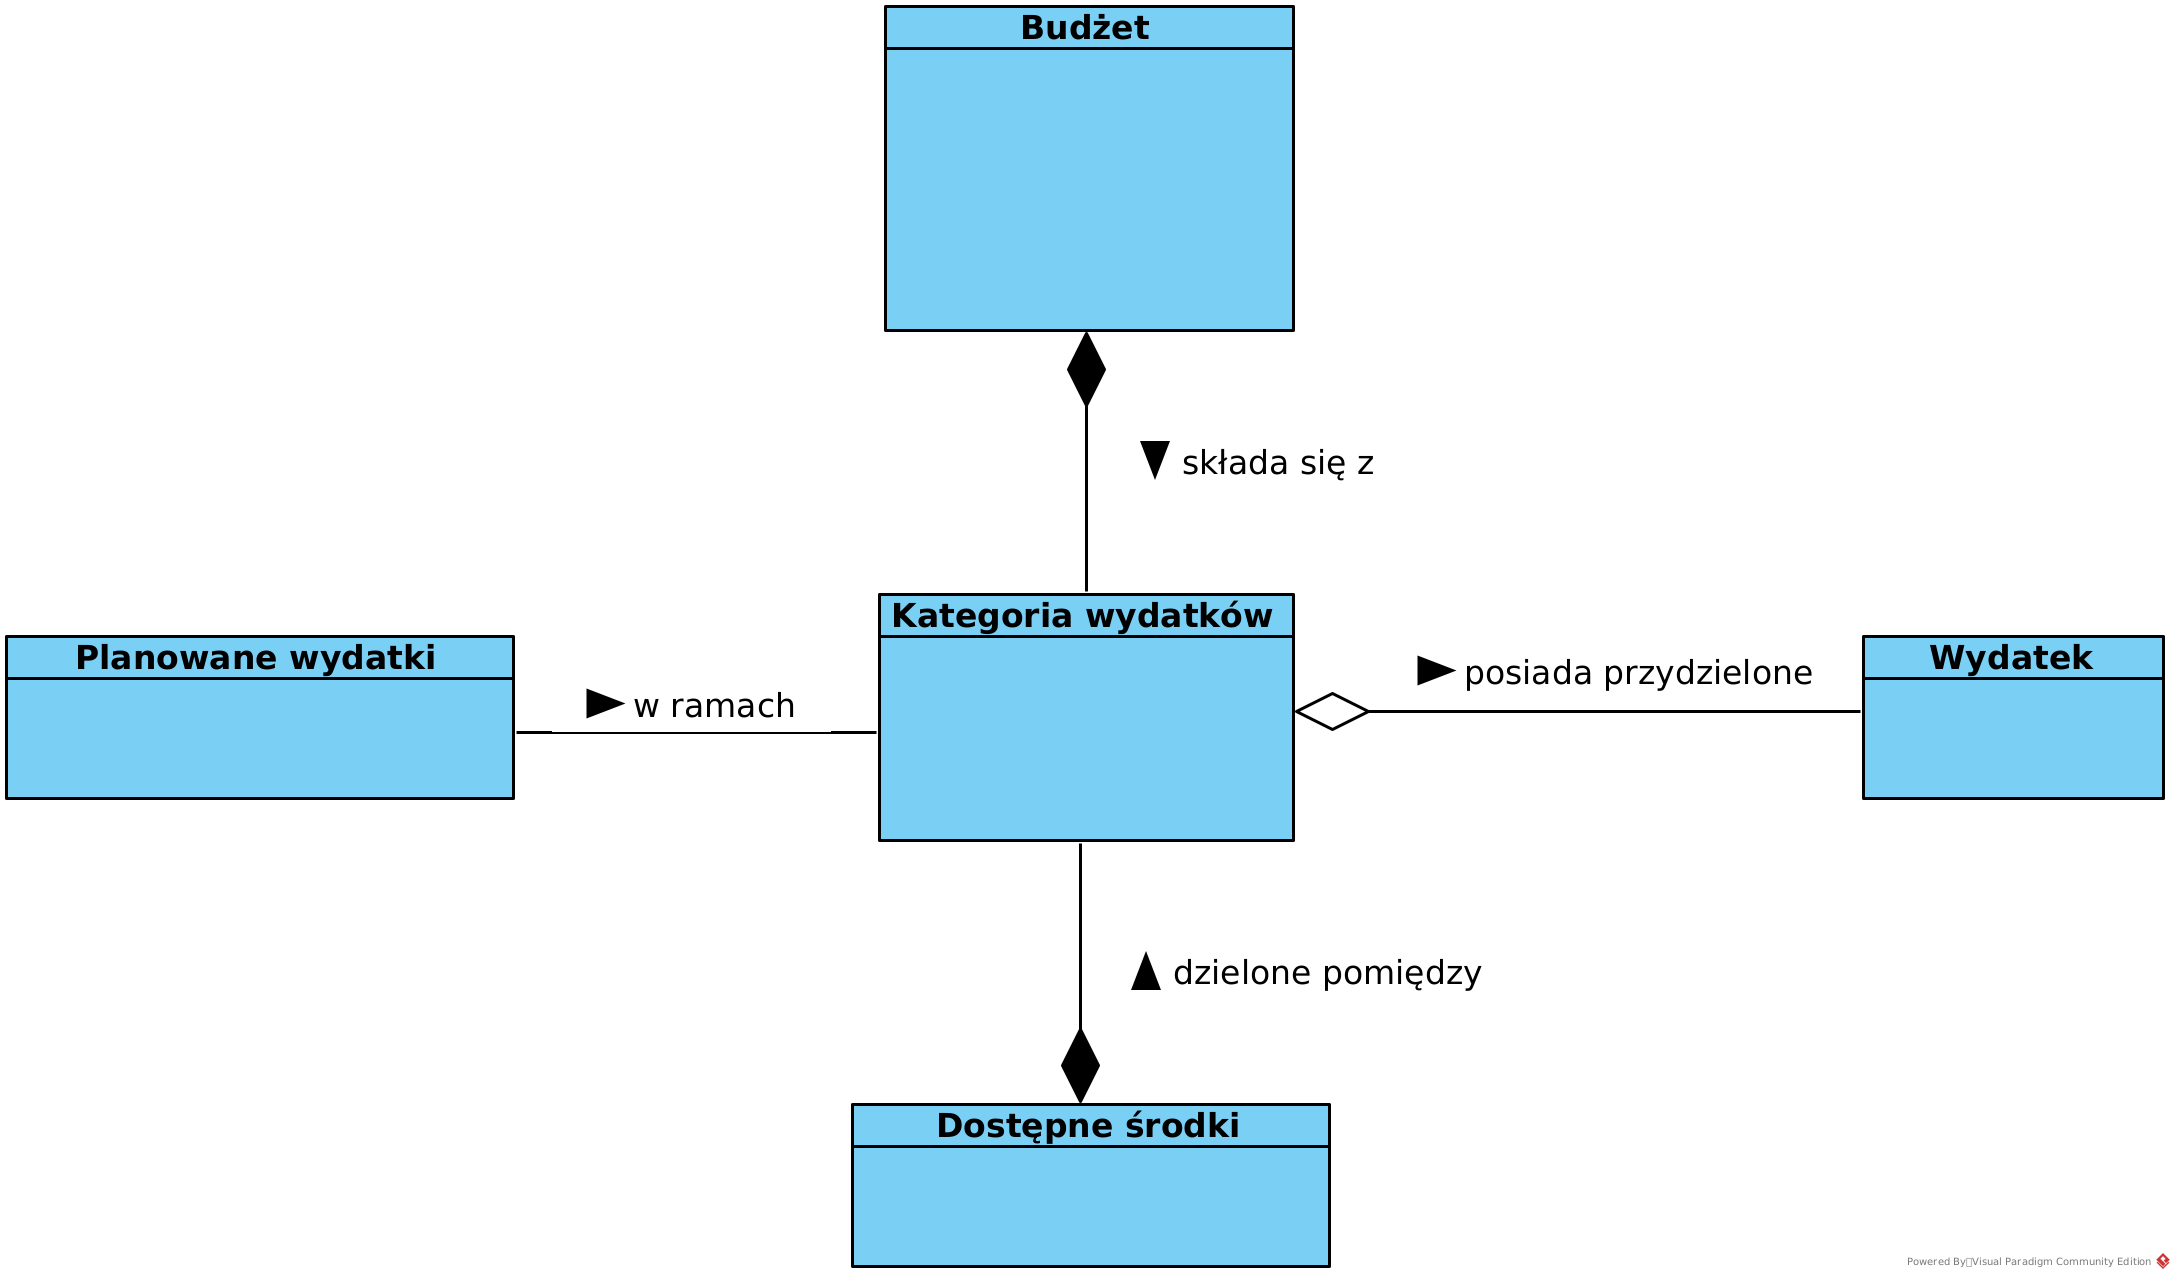
\includegraphics[scale=0.75]{domain-model.png}
	\caption{Model przedstawiający zagadnienia budżetu osobistego na diagramie UML}
	\label{fig:domain-model}
\end{figure}

Jak wcześniej wspomniałem, w pracy tej zająłem się opracowaniem rozwiązania dla zagadnienia prowadzenia budżetu osobistego. Można jednak użyć podanego wyżej modelu, aby poradzić sobie także z prowadzeniem budżetu domowego. Rozważmy sytuację, w której budżet domowy chce prowadzić mieszkająca razem rodzina. W takim przypadku dostępnymi środkami mogą być zarobki rodziców. Stworzą oni kategorie dla wszystkich wydatków wymaganych do prowadzenia domu rodzinnego, oszczędzania, czy też oddzielne na tzw. kieszonkowe dla dzieci. Jeśli budżet domowy chcieliby prowadzić np. mieszkający razem studenci, dostępnymi środkami byłyby składki każdego z nich na wspólny budżet. Mogliby oni stworzyć kategorie dla wydatków dotyczących prowadzenia wspólnego domu takie jak czynsz, artykuły gospodarstwa domowego, opłaty za telewizję, Internet itd.

Z jednej strony budżet osobistego wymaga poświęcenia dodatkowego czasu na stworzenie oraz jego regularne prowadzanie. Z drugiej strony możemy w zamian liczyć na większą kontrolę nad stanem naszego portfela. Przy założeniu, że taki budżet prowadzony jest regularnie, mamy wiedzę o tym, ile pieniędzy możemy jeszcze wydać. Może to pozwolić nawet na uniknięcie długów. Osoba prowadząca budżet osobisty i historię wydatków może także łatwiej analizować swoje nawyki konsumenckie oraz je poprawiać, aby móc efektywniej zarządzać swoimi pieniędzmi w przyszłości.
\bigbreak
Zdecydowałem się na stworzenie aplikacji, która będzie dostarczała  podstawowe funkcjonalności do zrealizowania opisanego wyżej zadania oraz będzie na tyle prosta, aby nowy użytkownik mógł jak najmniejszym kosztem zacząć prowadzić swój budżet osobisty. W dalszej części pracy opisałem jakie funkcje udostępnia aplikacja. Następnie skupiłem się na przedstawieniu i uzasadnieniu mojego rozwiązania pod względem technologicznym. W końcowej części pracy podsumowałem zrealizowane zadania oraz podałem przykłady sposobów na dalsze ulepszenie aplikacji.

\section{Przykłady innych rozwiązań}
Użytkownicy zainteresowani tematyką prowadzenia budżetu osobistego mają duży wybór dostępnych rozwiązań. Istnieją zarówno aplikacje dostępne przez przeglądarkę, tradycyjne programy i aplikacje na urządzenia mobilne. Wiele programów dostępnych jest jednocześnie na wielu rodzajach urządzeń dla wygody użytkowników. Ja skupiłem się na rozwiązaniach, które dostępne są przez przeglądarkę, gdyż są najbardziej zbliżone do rozwiązania proponowanego przeze mnie.
\subsection{You Need a Budget (YNAB)}
Aplikacja You Need a Budget \citep{ynab} jest dostępna przez przeglądarkę internetową oraz w postaci aplikacji na urządzenia mobilne na systemy operacyjne Android i iOS. Jest to program płatny, który kosztuje 14,99\$ miesięcznie lub 89,99\$ rocznie \cite{ynab-price}. Ideą tej aplikacji jest nie tyle zautomatyzowanie całego procesu zarządzania budżetem i całkowite wyręczenie użytkownika, co nauczenie go jak taki budżet tworzyć, więc aplikacja YNAB wymaga od użytkownika poświęcenia czasu na ręczne tworzenie budżetu. Filozofia tworzenia budżetu osobistego w tej aplikacji polega na rozdzieleniu pieniędzy co do grosza na nasze cele. Program ten posiada użyteczną funkcję automatycznego pobierania wydatków z konta bankowego.

\subsection{Mint}
Mint \cite{mint} to darmowy program dostępny przez przeglądarkę internetową oraz jako aplikacja na urządzenia mobilne na systemy operacyjne Android i iOS. Aplikacja dostępna jest za darmo, ale wyświetla użytkownikom reklamy ofert od swoich partnerów biznesowych. To rozwiązanie posiada wiele funkcji automatyzujących cały proces zarządzania budżetem. Automatycznie pobiera wydatki z połączonego konta bankowego i przypisuje je do odpowiednich kategorii. Posiada też dodatkowe funkcje oprócz prowadzenia budżetu takie jak przypominanie o płatnościach za subskrypcje i rachunki lub wysyłanie użytkownikom porad, jak mogą lepiej zarządzać pieniędzmi. Dostępne są także informacje o zdolności kredytowej, funkcje związane z inwestowaniem oraz inne funkcjonalności dotyczące pieniędzy. Mamy więc tutaj więcej funkcji niż w poprzednim rozwiązaniu.
\begin{figure}
\centering
\begin{subfigure}{0.45\textwidth}
    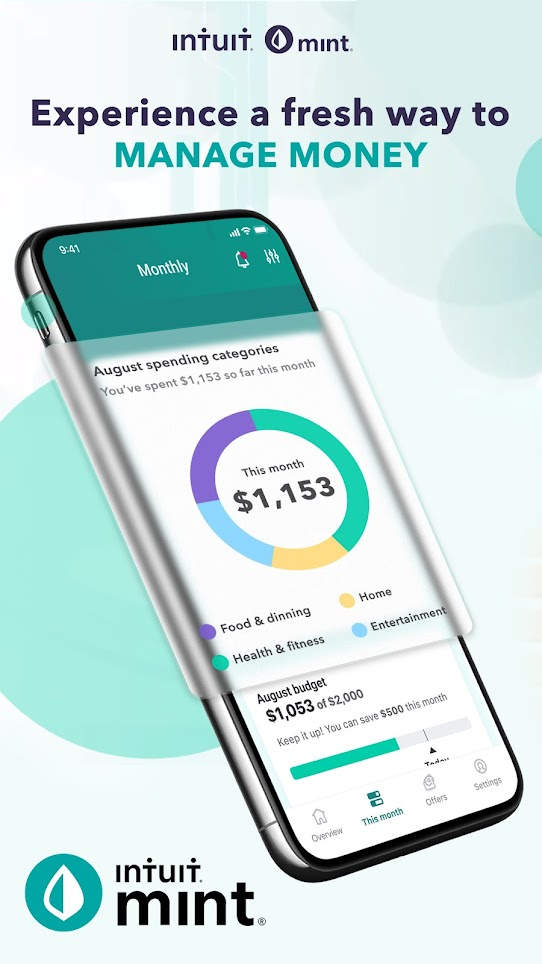
\includegraphics[width=\textwidth]{mint-screen.jpg}
    \caption{Mint}
    \label{fig:mint}
\end{subfigure}
\hfill
\begin{subfigure}{0.45\textwidth}
    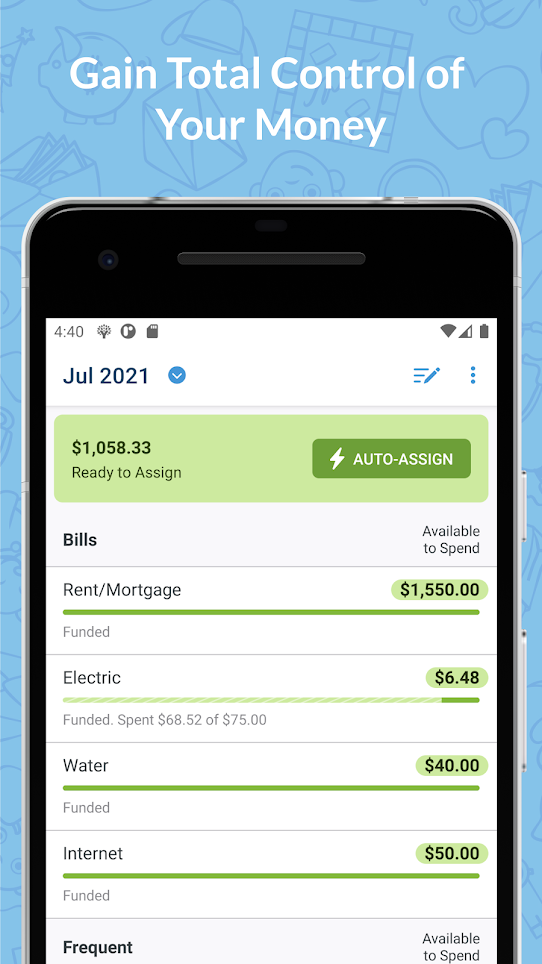
\includegraphics[width=\textwidth]{ynab.png}
    \caption{You Need A Budget}
    \label{fig:ynab}
\end{subfigure}     
\caption{Inne rozwiązania dotyczące prowadzenia budżetu osobistego}
\label{fig:mint-ynab}
\end{figure}
\chapter{Opis systemu}
\section{Sposób instalacji i dostępu do systemu}
\subsection*{Część serwerowa}
Część serwerowa wymaga do uruchomienia programu PostgreSQL \citep{pgsql} w wersji 13.4 oraz Java Runtime Enviroment (JRE) \citep{java} w wersji 17.0.1.
Część serwerowa została już zbudowana i dostępna jest w postaci pliku JAR, w którym zawarty jest wbudowany serwer aplikacji Tomcat.

\subsubsection*{Samodzielne budowanie aplikacji}
Źródła programu dostępne są w repozytorium Git \citep{git} na stronie Github \citep{github} pod adresem \url{https://github.com/mat-kmita/budget-manager} i możemy ich użyć, jeśli chcemy samodzielnie zbudować program.
\noindent Do pobrania plików źródłowych możemy użyć na przykład polecenia:
\begin{lstlisting}[language=bash]
  $ git clone https://github.com/mat-kmita/budget-manager.git
\end{lstlisting}
Do zbudowania programu wymagane jest narzędzie Gradle \citep{gradle}.
\noindend Aby zbudować program należy w katalogu \path{thesis_project} z plikami źrodłowymi części serwerowej wykonać:
\begin{lstlisting}[language=bash]
  $ gradle bootJar
\end{lstlisting}

\subsubsection*{Przygotowanie bazy danych}
Program wymaga stworzenia bazy danych PostgreSQL. Potrzebujemy do tego użytkownika bazy danych.
\noindend  Żeby go stworzyć użyjemy narzędzia createuser \citep{pgsql-createuser}:
\begin{lstlisting}[language=bash]
  $ createuser -d -P -h localhost -p 5432 -U postgres -W thesis
\end{lstlisting}
Program zapyta wtedy o hasło dla tworzonego użytkownika, które należy podać i zapamiętać. Nazwa użytkownika to thesis, ale można ją dostosować według własnego uznania przy czym będzie to wymagało zmiany konfiguracji aplikacji. Opcja h ustawia nazwę hosta, na którym działa baza danych, opcja p ustawia port, na którym baza nasłuchuje, opcja U ustawia istniejącego użytkownika bazy, jako który chcemy wykonać to polecenie. Opcje należy dostosować zgodnie z lokalną konfiguracją.
Następnym krokiem jest już stworzenie bazy danych.
\noindend  Użyjemy do tego narzędzia createdb \citep{pgsql-createdb}:
\begin{lstlisting}[language=bash]
  $ createdb -h localhost -p 5432 -O thesis -U thesis thesis_db    
\end{lstlisting}
Podobnie jak wyżej opcje h i p odpowiadają za ustalenie adresu bazy danych. Opcja O ustawia stworzonego wcześniej użytkownika jako właściciela bazy. W powyższym poleceniu nadajemy bazie nazwę thesis$\_$db, ale możemy to dostosować pamiętając, że będzie to wymagało zmiany domyślnej konfiguracji aplikacji.

\subsubsection*{Konfiguracja aplikacji}
Aplikacja konfigurowana jest przez plik konfiguracyjny \path{application.properties}. Znajduje się ona w źródłach aplikacji w katalogu \path{thesis_project/src/main/resources/application.properties}. Możemy dostosować opcje w tym pliku zanim zbudujemy aplikację. Jeśli aplikacja jest już zbudowana, możemy umieścić w katalogu, w którym znajduję się plik JAR plik o nazwie \path{application.properties}, który będzie nadpisywał domyślne opcje. 
Przed uruchomieniem aplikacji należy ustawić hasło użytkownika bazy danych. W pliku konfiguracyjnym należy wpisać:
   \begin{lstlisting}
spring.datasource.password=<hasło użytkownika bazy danych>
	\end{lstlisting}
Jeśli użyliśmy niestandardowej nazwy użytkownika należy także zmienić opcję:
	\begin{lstlisting}
spring.datasource.username=<nazwa użytkownika bazy danych>
	\end{lstlisting}
Jeśli chcemy zmienić hosta, port lub nazwę bazy danych, z którą aplikacja ma się łączyć powinniśmy zmodyfikować opcję:
	\begin{lstlisting}
spring.datasource.url=<adres bazy danych>
	\end{lstlisting}
Format adresu bazy danych opisany jest na stronie internetowej \url{https://www.postgresql.org/docs/current/libpq-connect.html#LIBPQ-CONNSTRING}.
Pozostałe opcje konfiguracji opisane są na stronie internetowej \url{https://docs.spring.io/spring-boot/docs/current/reference/html/application-properties.html}.

\subsubsection{Uruchamianie programu}
Gdy skończyliśmy konfigurację aplikacji dla naszego środowiska, możemy ją uruchomić. 
\noindend W katalogu, w którym znajduje się plik JAR o nazwie \path{application.jar} wykonujemy polecenie:
\begin{lstlisting}[language=bash]
  $ java -jar application.jar
\end{lstlisting}
Taki plik dostępny jest już w głównym katalogu projektu.

\subsection*{Część kliencka}
Do uruchomienia części klienckiej wymagane jest Node.js \citep{nodejs} w wersji 17.0.1 oraz npm \citep{npm} w wersji 8.3.2.

Aplikacja została już zbudowana i jest gotowa do uruchomienia. Kod źródłowy znajduje się w katalogu \path{thesis-front-end}.
\noindend  Będąc w tym katalogu należy wykonać polecenia:
\begin{lstlisting}[language=bash]
  $ npm install -g serve
  $ serve -s build
\end{lstlisting}
Aplikacja zostanie uruchomiona i będzie nasłuchiwała na porcie 3000.

\section{Wymagania funkcjonalne}
\begin{itemize}
	\item Udostępnianie użytkownikowi gotowego zestawu kategorii wydatków do podziału budżetu.
	\item Możliwość dodawania nowych kategorii przez użytkownika.
	\item Możliwość zmiany nazwy kategorii.
	\item Możliwość usuwania istniejących kategorii.
	\item Możliwość podziału portfela na konta odpowiadające rzeczywistym kontom użytkownika lub będące wirtualnym podziałem środków.
	\item Możliwość edycji właściwości konta oraz usuwania konta.
	\item Możliwość transferu środków pomiędzy kontami wraz zapisem informacji dodatkowych o transferze, takich jak: data jego przeprowadzenia, komentarz.
	\item Możliwość edycji danych zarejestrowanego transferu i całkowitego usunięcia go.
	\item Możliwość rejestracji przychodów i wydatków wraz z informacjami takimi jak: data operacji, kwota, kategoria, komentarz, płatnik.
	\item Możliwość edycji informacji o przychodach i wydatkach oraz usuwania tych operacji.
	\item Możliwość tworzenia budżetów poprzez przydzielanie dostępnych środków pomiędzy istniejące kategorie.
	\item Możliwość zmiany środków przydzielonych do kategorii w ramach budżetu.
	\item Możliwość wyświetlania budżetu w postaci listy kategorii wraz z informacjami o sumie środków w ramach każdej kategorii wydanej oraz dostępnymi jeszcze środkami.
	\item Możliwość wyświetlania informacji o sumie środków wydanych każdego dnia z danego przedziału czasowego.
	\item Możliwość wyświetlania statystyk o procentowym udziale wydatków w każdej kategorii we wszystkich wydatkach.
\end{itemize}

\section{Wymagania niefunkcjonalne}
\begin{itemize}
	\item Interfejs graficzny aplikacji powinien być intuicyjny, spójny i prosty w obsłudze.
	\item Aplikacja powinna sprawdzać poprawność danych wprowadzanych przez użytkownika.
	\item Błędy w działaniu aplikacji powinny być przekazywane użytkownikowi z prostym i zrozumiałem wytłumaczeniem, nieudostępniając informacji o wewnętrznym działaniu aplikacji.
	\item Dostęp do bazy danych musi być chroniony przed nieuprawnionymi osobami.
\end{itemize}
\section{Opis funkcji systemu}
Koncepcja aplikacji polega na założeniu, że użytkownik będzie samodzielnie regularnie rejestrował w aplikacji wszystkie swoje wydatki oraz wpływy oraz ręcznie tworzył budżet rozdzielając pieniądze pomiędzy różne kategorie. Program będzie te informacje zapisywał oraz obliczał środki dostępne w ramach budżetu.

Poniżej wytłumaczyłem podstawowe pojęcia używane w aplikacji.
\begin{itemize}
	\item \textbf{Transakcje} - operacje pieniężne, które są wydatkami lub wpływami z zewnętrznych źródeł. Te operacje mogą wpływać na stan budżetu.
	\item \textbf{Transfery} - operacje pieniężne pomiędzy dwoma różnymi kontami, które nie wpływają na budżet, ale dotyczą przeniesienia środków wewnątrz portfela użytkownika
		\item \textbf{Kategoria transakcji} - podział wszystkich transakcji na różne kategorie dotyczące tej samej dziedziny. Ocena do jakiej kategorii należy transakcja leży całkowicie po stronie użytkownika.
	\item \textbf{Budżet} - budżet to comiesięczny podział wpływów pomiędzy różne kategorie wraz z wydatkami w tym miesiącu oraz informacją o środkach dostępnych jeszcze w ramach każdej z kategorii.

\end{itemize}
\subsection{Zarządzanie kontami}
Użytkownik posiada możliwość podziału swojego portfela na różne konta. Ta funkcja pozwala śledzić ilość pieniędzy ulokowanych w różnych źródłach. Dla wygody użytkownika konta są podzielone pomiędzy cztery różne rodzaje: rozliczeniowe, oszczędnościowe, gotówkę oraz inne. Lista kont wyświetlana jest w panelu nawigacyjnym po lewej stronie ekranu. Możemy stamtąd przejść do listy transakcji lub transferów przypisanych do każdego z kont. Na górze strony będą wtedy wyświetlane informacje o koncie, którego ekran dotyczy. Znajdziemy tam nazwę konta, opis, rodzaj i aktualny stan środków na koncie. Obok tych informacji znajdują się przyciski ``Delete account'' oraz ``Edit account'' służące do usuwania konta i edycji danych o nim. Aby dodać nowe konto należy nacisnąć na przycisk ``Create new account'' w panelu nawigacyjnym. Wyświetla się wtedy formularz, w którym należy podać nazwę i rodzaj konta oraz opcjonalnie opis i początkowy stan tego konta.
\begin{figure}
	\centering
	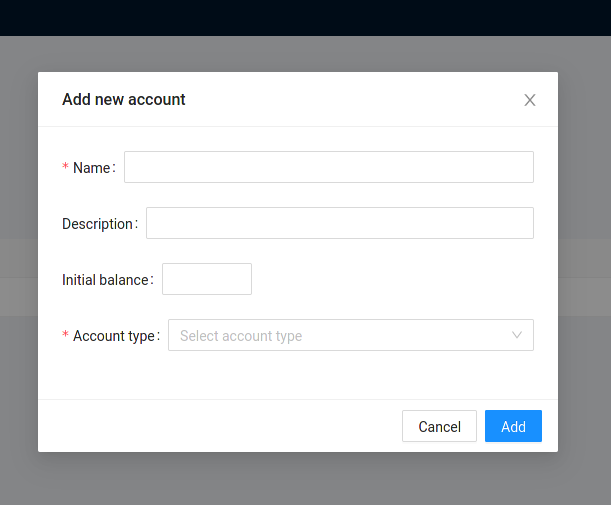
\includegraphics[scale=0.7]{screen-new-account.png}
	\caption{Formularz tworzenia nowego konta}
	\label{fig:screen-new-account}
\end{figure}
\begin{figure}
	\centering
	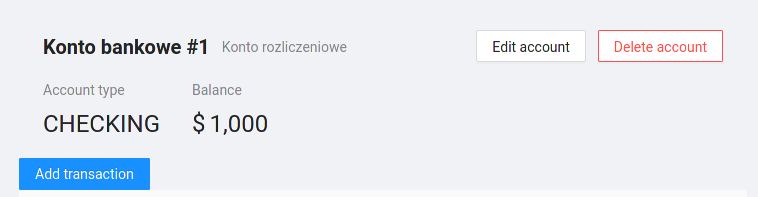
\includegraphics[scale=0.7]{screen-panel-info-konto.png}
	\caption{Widok informacji o koncie}
	\label{fig:screen-account-info}
\end{figure}
\subsection{Wyświetlanie operacji}
Aby wyświetlić operacje danego typu należy w panelu nawigacyjnym po lewej stronie wybrać ``Transactions'' lub ``Transfers'' dla jakiegoś konta. Zostanie wtedy wyświetlona tabela z transakcjami lub transferami dotyczącymi tego konta. Operacje posortowane są według daty ich wykonania od najnowszych do najstarszych. Dla każdej transakcji wyświetlane są: identyfikator tej operacji, data wykonana, odbiorca płatności (lub nadawca dla przychodów), kategoria, opis, kwota, przycisk otwierający okienko modyfikacji operacji i przycisk usuwający operację. Dla transferów wyświetlane są: identyfikator transferu, data wykonania, nazwa drugiego konta, opis oraz kwota. Dane w tabeli podzielone są na strony. Użytkownik może się między nimi przemieszczać używając przycisków z numerem strony lub wpisując numer dowolnej strony, do której chce przejść. Ilość elementów na stronie może zostać wybrana spomiędzy 10, 20, 50, 100.
\begin{figure}
	\centering
	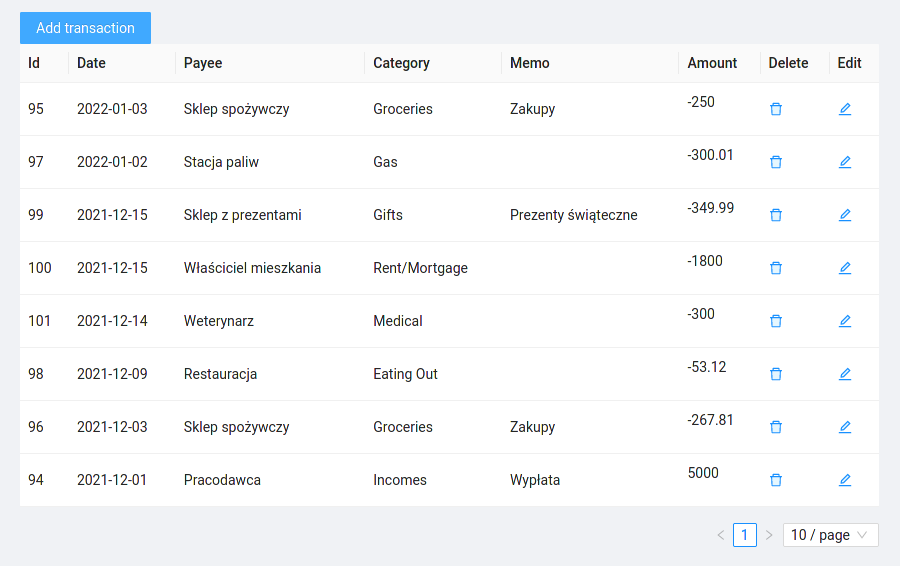
\includegraphics[scale=0.6]{screen-transactions-list.png}
	\caption{Tabela przedstawiająca transakcje dla danego konta}
	\label{fig:screen-transactions-list}
\end{figure}
\begin{figure}
	\centering
	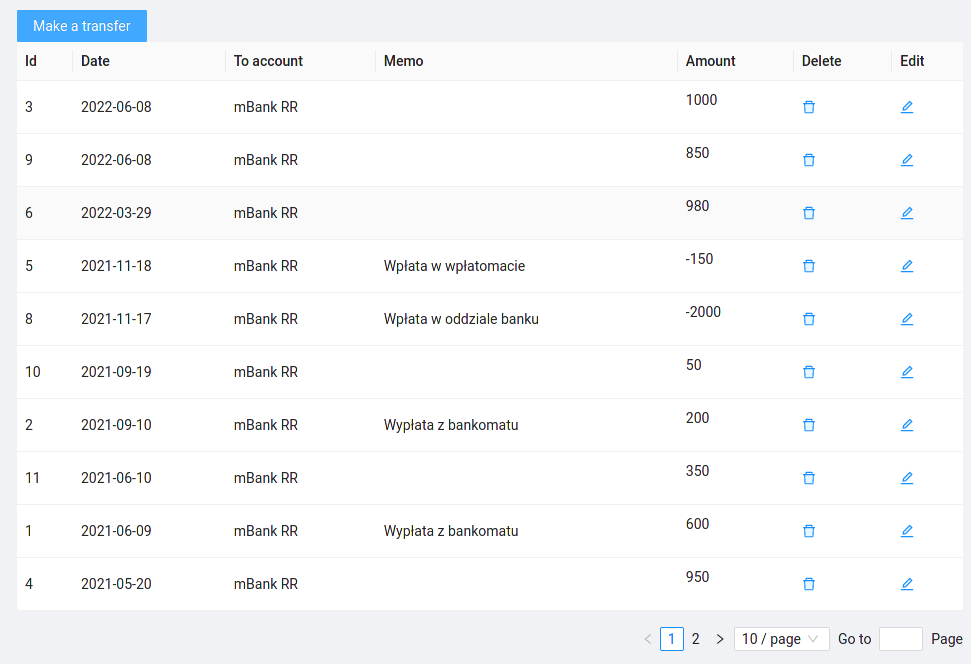
\includegraphics[scale=0.55]{screen-transfers-list.png}
	\caption{Tabela przedstawiająca transfery dla danego konta}
	\label{fig:screen-transfers-list}
\end{figure}
\subsection{Rejestrowanie operacji}
Zgodnie z koncepcją aplikacji, użytkownik powinien regularnie rejestrować w programie swoje wydatki, przychody i transfery pieniędzy. Aby to zrobić, należy nacisnąć na przycisk ``Add transaction'' lub ``Make a transfer''. Są one widoczne na ekranach transakcji i transferów dla danego konta. Pierwszy z nich służy do rejestrowania transakcji, a drugi do przenoszenia środków na inne konto. Naciśnięcie tych przycisków powoduje wyświetlenie okienka z formularzem. Należy w nim podać dane o operacji. Niektóre pola są wymagane i oznaczone są one znakiem czerwonej gwiazdki. Pozostałe pola są opcjonalne.
\begin{figure}
	\centering
	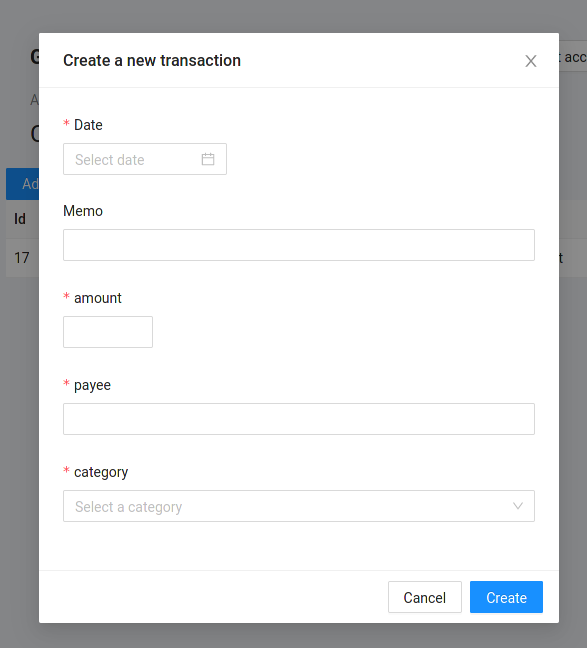
\includegraphics[scale=0.7]{screen-new-transaction-form.png}
	\caption{Formularz dodawania nowej transakcji}
	\label{fig:screen-new-transaction}
\end{figure}
\begin{figure}
	\centering
	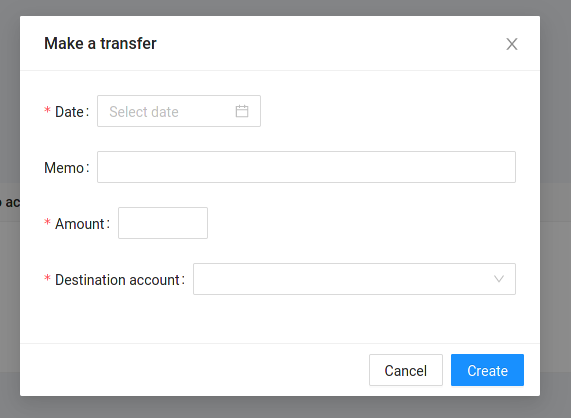
\includegraphics[scale=0.7]{screen-make-transfer.png}
	\caption{Formularz dodawania nowego transferu pomiędzy kontami}
	\label{fig:screen-make-transfer}
\end{figure}
\subsection{Modyfikacja i usuwanie operacji}
Przy każdej operacji znajdują się przyciski pozwalające na jej edycję lub usunięcie. Naciśnięcie przycisku do edycji operacji spowoduje wyświetlenie okienka z formularzem, w którym możemy zmienić dane operacji a następnie je zapisać. Naciśnięcie przycisku do usuwania operacji spowoduje wyświetlenie okienka, w którym należy usunięcie potwierdzić lub anulować. Ma to za zadanie chronić przed przypadkowym usuwaniem operacji.
\begin{figure}
	\centering
	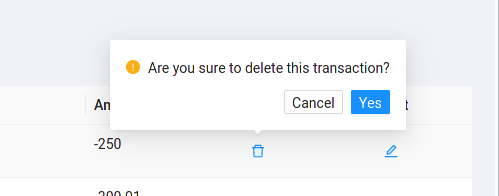
\includegraphics[scale=0.7]{screen-delete-transaction.png}
	\caption{Potwierdzenie usunięcia operacji}
	\label{fig:screen-delete-transaction}
\end{figure}
\begin{figure}
	\centering
	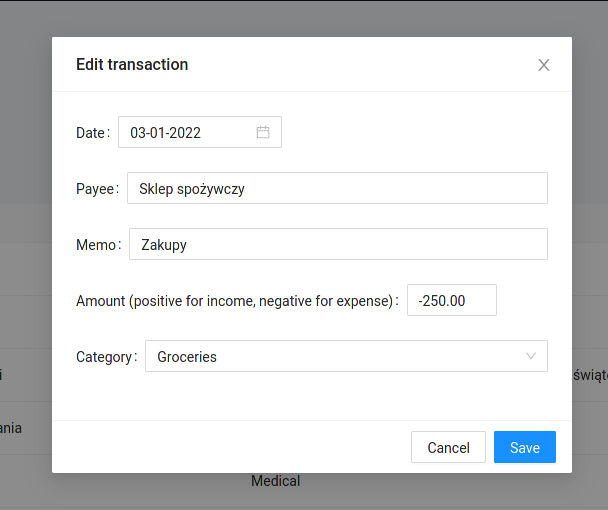
\includegraphics[scale=0.7]{screen-edit-transaction.png}
	\caption{Okienka z formularzem do edycji transakcji}
	\label{fig:screen-edit-transaction}
\end{figure}

\subsection{Wyświetlanie budżetów}
Naciśnięcie na przycisk "Budget" w panelu nawigacyjnym powoduje przejście do widoku budżetu. Początkowo wyświetlany jest budżet dla aktualnego miesiąca. W górnej części tej strony umieszczone są przyciski służące do zmieniania miesiąca. Widoczna jest tam też kwota, która nie została jeszcze rozdzielona w ramach budżetu i możemy ją rozdysponować pomiędzy kategorie. Poniższy kod pochodzący z kodu źródłowego aplikacja oblicza tę kwotę (pominięto nieistotne fragmenty):
\begin{lstlisting}
/**
 * Calculate amount available to budget
 */
public int available() {
    Budget previousBudget = this.getPreviousBudget();
    int overSpentAmount = 0; // Amount overspent in all categories for previous budget. Should be negative
    int previousBudgetAvailable = 0; // Amount available to budget in previous budget

    if (previousBudget != null) {
    	previousBudgetAvailable = previousBudget.available();
        overSpentAmount = previousBudget.getBudgetCategories()
                .stream()
                .map(BudgetCategory::available)
                .filter(i -> i < 0)
                .reduce(0, Integer::sum);
	}
	
	// Sum amount already budgeted this month
    int budgetedAmount = this.getBudgetCategories()
            .stream()
            .map(BudgetCategory::getAmount)
            .reduce(0, Integer::sum);
            
    // Incomes for this month        
    int incomesSum = this.getBudgetCategories()
            .stream()
            .filter(x -> x.getCategory().getId() == 1)
            .getSpent();

    return previousBudgetAvailable + incomesSum + overSpentAmount - budgetedAmount;
}
\end{lstlisting}
W budżecie dostępne mamy środki pochodzące z kategorii \texttt{Incomes} w danym miesiącu. Środki nie rozdzielone w ramach budżetu na dany miesiąc przechodzą na kolejny. Dodatkowo wszystkie wydatki ponad zaplanowane w poprzednim miesiącu są odejmowane od następnego budżetu. 
Budżet przedstawiony jest w postaci tabeli, która zawiera listę kategorii oraz kolumny z informacją o kwocie rzeczywiście wydanej w ramach tej kategorii, kwocie zaplanowanej do wydania oraz dostępnych nadal środkach. Jeśli ilość środków wydanych w ramach kategorii jest dodatnia to przychody w tej kategorii były większe niż wydatki. Jeśli ilość dostępnych środków jest ujemna to wydano więcej niż pozwala na to budżet. Naciśnięcie przycisku w kolumnie z zaplanowaną do wydanie kwotą powoduje wyświetlenie formularza, w którym można tę kwotę zmienić. Środki dostępne w ramach kategorii liczone są przez następujący kod:
\begin{lstlisting}
/**
 * Calculate amount available to spent in this budgeting category
 */
public int available() {
        int previousMonthAvailable = Optional.ofNullable(this // May be null if this is first budget
                .getBudget()
                .getPreviousBudget())
                .map(Budget::getBudgetCategories)
                .orElse(List.of())
                .stream()
                .filter(x -> Objects.equals(x.getCategory().getId(), this.getCategory().getId()))
                .map(BudgetCategory::available)
                .findFirst()
                .orElse(0);

        // Ignore overspent categories
        if (previousMonthAvailable < 0) {
            previousMonthAvailable = 0;
        }

        return previousMonthAvailable + this.amount + this.getSpent();
    }
\end{lstlisting}
Wynika z niego, że środki, których nie wydamy w danym miesiącu przechodzą na kolejny miesiąc.
\begin{figure}
	\centering
	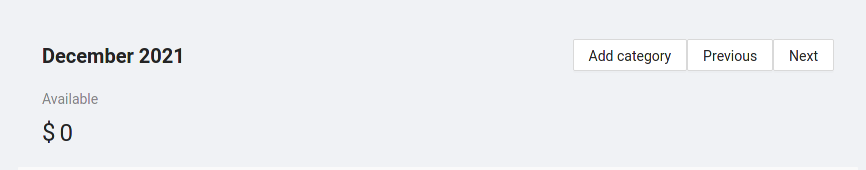
\includegraphics[scale=0.65]{screen-budget-header.png}
	\caption{Nagłówek ekranu budżetu}
	\label{fig:screen-budget-header}
\end{figure}
\begin{figure}
	\centering
	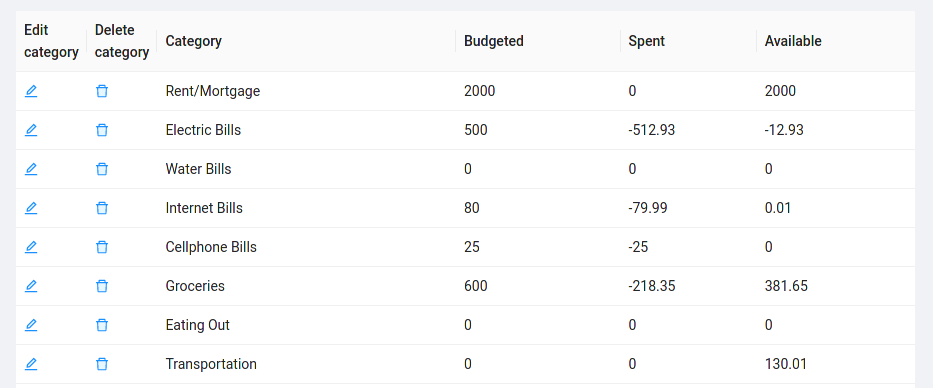
\includegraphics[scale=0.62]{screen-budget-table.png}
	\caption{Widok budżetu w postaci tabeli}
	\label{fig:screen-budget-table}
\end{figure}
\begin{figure}
	\centering
	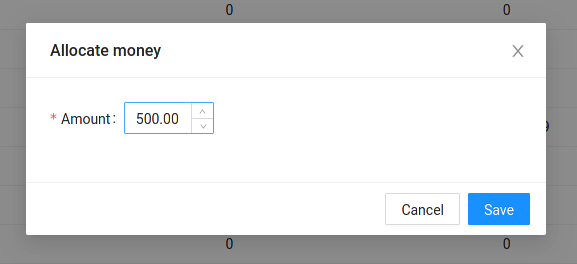
\includegraphics[scale=0.7]{screen-budgeting-form.png}
	\caption{Formularz planowania kwoty do wydania w ramach kategorii}
	\label{fig:screen-budget-amount}
\end{figure}
\subsection{Zarządzanie kategoriami}
Na ekranie budżetu możemy także zarządzać kategoriami budżetowymi. W nagłówku widoku budżetu znajduje się przycisk ``Add category'', którego naciśnięcie powoduje wyświetlenie formularza do wpisania danych kategorii. W tabeli prezentującej stan budżetu dla każdej z kategorii dwie pierwsze kolumny zawierają przyciski do edycji i usuwania kategorii.Naciśnięcie przycisku edycji także powoduje wyświetlenie formularza. Usuwanie kategorii nie następuje od razu po naciśnięciu przycisku, gdyż należy jeszcze tę operację potwierdzić.
\begin{figure}
\centering
	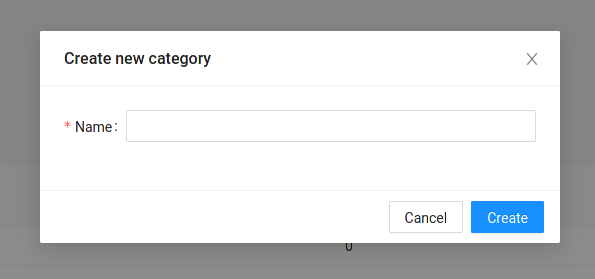
\includegraphics[scale=0.7]{screen-category-add-form.png}
	\caption{Formularz tworzenia nowej kategorii budżetowej}
	\label{fig:screen-heatmap}
\end{figure}
\subsection{Wyświetlanie statystyk}
Aplikacja udostępnia użytkownikom możliwość przeglądania raportów dotyczących budżetu przedstawionych w postaci diagramów. Strona raportów dostępna jest po wybraniu ``Reports'' z panelu nawigacyjnego. Różne rodzaje statystyk dostępne są poprzez wybór odpowiedniej zakładki.

W zakładce ``Heat map'' udostępniony jest raport dotyczący dziennych wydatków i przychodów. Dzięki niemu użytkownik ma możliwość szybkiego zobaczenia jak duże są wydatki lub przychody każdego dnia. Pokazywany jest on w postaci diagramu heatmap. Każdy kafelek reprezentuje jeden dzień, a jego kolor zależny jest od kwoty w danym dniu. Im ciemniejszy, tym jest ona większa. Domyślnie pokazywane są dane z ostatnich 12 miesięcy. Użytkownik może wyświetlić raport dotyczący wybranego przez siebie roku poprzez użycie formularza wyboru roku znajdującego się nad diagramami. Obok tego formularza znajduje się przycisk poprzez który można znowu wyświetlić dane dla ostatnich 12 miesięcy.
\begin{figure}
\centering
	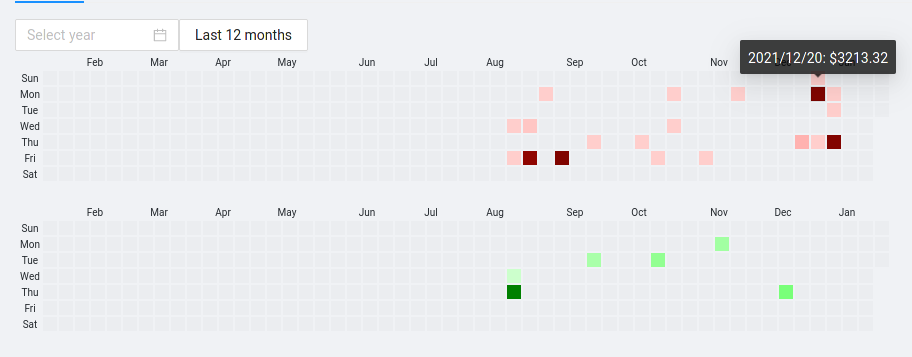
\includegraphics[scale=0.5]{screen-heatmap.png}
	\caption{Raport sumy wydatków i przychodów dziennych}
	\label{fig:screen-heatmap}
\end{figure}

W zakładce ``Expenses by category'' udostępniony jest raport przedstawiający graficznie procentowy udział wydatków z każdej kategorii, który pomaga analizować na co przeznaczane są środki. Użytkownik ma możliwość wyboru zakresu dat z jakich mają być brane pod uwagę transakcje. Domyślnie pokazywany jest diagram dla transakcji z aktualnego miesiąca.
\begin{figure}
\centering
	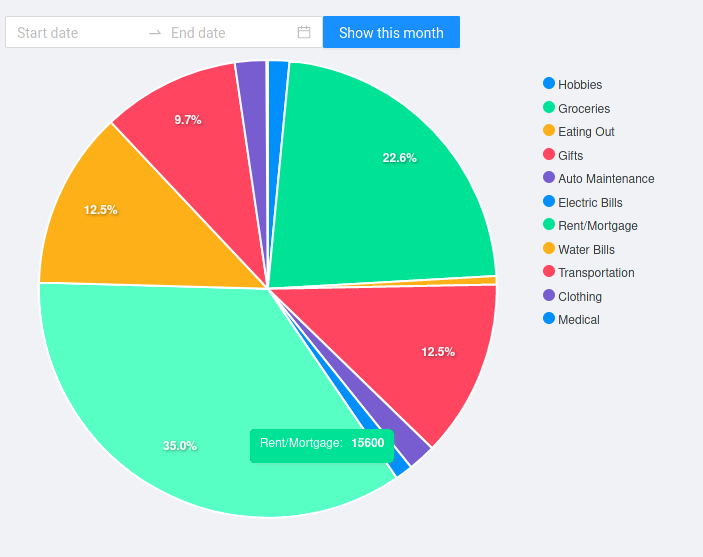
\includegraphics[scale=0.65]{screen-expenses-chart.png}
	\caption{Raport wydatków przypadających na kategorie}
	\label{fig:screen-expenses-chart}
\end{figure}

\chapter{Użyte rozwiązania technologiczne}
Program został podzielony na dwie części. Pierwsza z nich to część serwerowa. Odpowiada ona za logikę programu i przechowywanie danych w trwałej pamięci. Druga część to część kliencka. Jej głównym zadaniem jest prezentacja danych otrzymanych od części serwerowej użytkownikowi. Komunikacja między nimi odbywa się przez protokół HTTP. W dalszej części tego rozdziału dokładniej obie te części programu.
\section{Część serwerowa}
Część serwerowa programu została napisana z użyciem języka Java. W kodzie źródłowym możemy wydzielić trzy warstwy. Pierwsza z nich to warstwa dostępu do danych. Ta część programu komunikuje się z bazą danych i tłumaczy jej relacyjny system typów na architekturę obiektową języka Java. Druga warstwa to tzw. warstwa serwisowa. Udostępnia ona główną logikę działania programu i komunikuje się z jednej strony z warstwą dostępu do danych, aby zapisywać informacje w trwałej pamięci, a z drugiej strony udostępnia wyższej warstwie zbiór dostępnych do wykonywania w ramach logiki programu operacji. Tą wyższą warstwą jest warstwa kontrolerów. Kontrolery to obiekty wyspecjalizowane do odbierania żądań ze świata zewnętrznego. Korzystają z warstwy serwisów, aby zlecone żądania wykonać.
Kontrolery udostępniają bezstanowy interfejs API dostępu do programu. Aplikacja stworzona jest z wykorzystaniem architektury Representational State Transfer (REST) \cite{rest} , więc udostępnia zasoby (zasobem jest np. konto, transakcja, budżet), na których można wykonywać operacje zdefiniowane przez protokół HTTP, które powodują zmianę stanu tych zasobów.
\subsection{Spring}
Główną technologią użytą w tworzeniu części serwerowej jest framework Spring \cite{spring}. Jest to obecnie najpopularniejszy framework do tworzenia aplikacji w języku Java \cite{spring-popularity}. Pod nazwą Spring kryje się tak naprawdę wiele różnych bibliotek. Cały framework podzielony jest więc na moduły rozwiązujące różne problemy \cite{spring-modules} takie jak udostępnianie kontenera Inversion of Control (IoC) \citep{ioc}, tworzenie aplikacji internetowych, tworzenie aplikacji dla środowiska rozporoszonego uruchamianych w chmurze, zabezpieczanie aplikacji, dostęp do baz danych i inne. Udostępnianie kontenera IoC jest jedną z głównych funkcji tego frameworka, a implementacja tego wzorca w postaci zasady Dependency Injection jest używana także w mojej aplikacji.

W moim rozwiązaniu użyłem między innymi modułu Spring MVC \cite{spring-mvc}, który używany jest w warstwie prezentacji danych. Dzięki temu rozwiązaniu mogłem z łatwością odczytywać żądania przesyłane do kontrolerów w aplikacji z zewnątrz przez protokół HTTP. Spring MVC bazuje na technologii Servlet API i ułatwia definiowanie zasobów w architekturze REST. Wystarczy stworzyć metody i zdefiniować jakie adresy i metody HTTP mają one obsługiwać. Spring MVC zajmie się za nas niskopoziomowymi kwestiami obsługi żądań takimi jak odbieranie danych, tłumaczenie ich na obiekty języka Java i wysyłanie odpowiedzi.

Aby ułatwić sobie tworzenie aplikacji użyłem także modułu Spring Boot \cite{spring-boot}. Spring Framework wymaga konfiguracji używanych elementów poprzez pliki XML, kod Java lub adnotacje w języku Java \citep{java-annotations}. Twórcy tej biblioteki zauważyli, że większość programistów wybiera przy tworzeniu programów podobne opcje konfiguracji biblioteki Spring. Aby ułatwić z nią pracę, Spring Boot automatyzuje proces konfiguracji, zarówno elementów dotyczących frameworka Spring jak i innych bibliotek, udostępniając zdefiniowane wcześniej konfiguracje tych elementów. Pozwala to o wiele szybciej rozpocząć tworzenie programów nieprzejmując się pisaniem konfiguracji dopóki nie będziemy mieli żadnych specyficznych wymagań. Dzięki temu będziemy mieli mniej powtarzalnego kodu w naszej aplikacji.
\subsection*{Dokumentacja API REST}
Dokumentacja interfejsu programistycznego w architekturze REST stworzona jest automatycznie w formacie OpenAPI \citep{openapi} z użyciem narzędzia Swagger UI \citep{swagger}, które na podstawie wygenerowanej specyfikacji OpenAPI udostępnia interfejs graficzny. Możemy tam zobaczyć wszystkie udostępnianie zasoby, format danych wejściowych i wyjściowych, a także wykonać zapytania do interfejsu. Interfejs Swagger UI dostępny jest domyślnie pod adresem \url{http://localhost:8080/swagger-ui.html}, natomiast specyfikacja w formacie OpenAPI dostępna jest pod adresem \url{http://localhost:8080/v3/api-docs/}. Narzędzie te pozwalają w łatwy i szybki sposób udokumentować stworzony interfejs REST bez pisania specjalnego kodu, który by za to odpowiadał.
\begin{figure}
\centering
	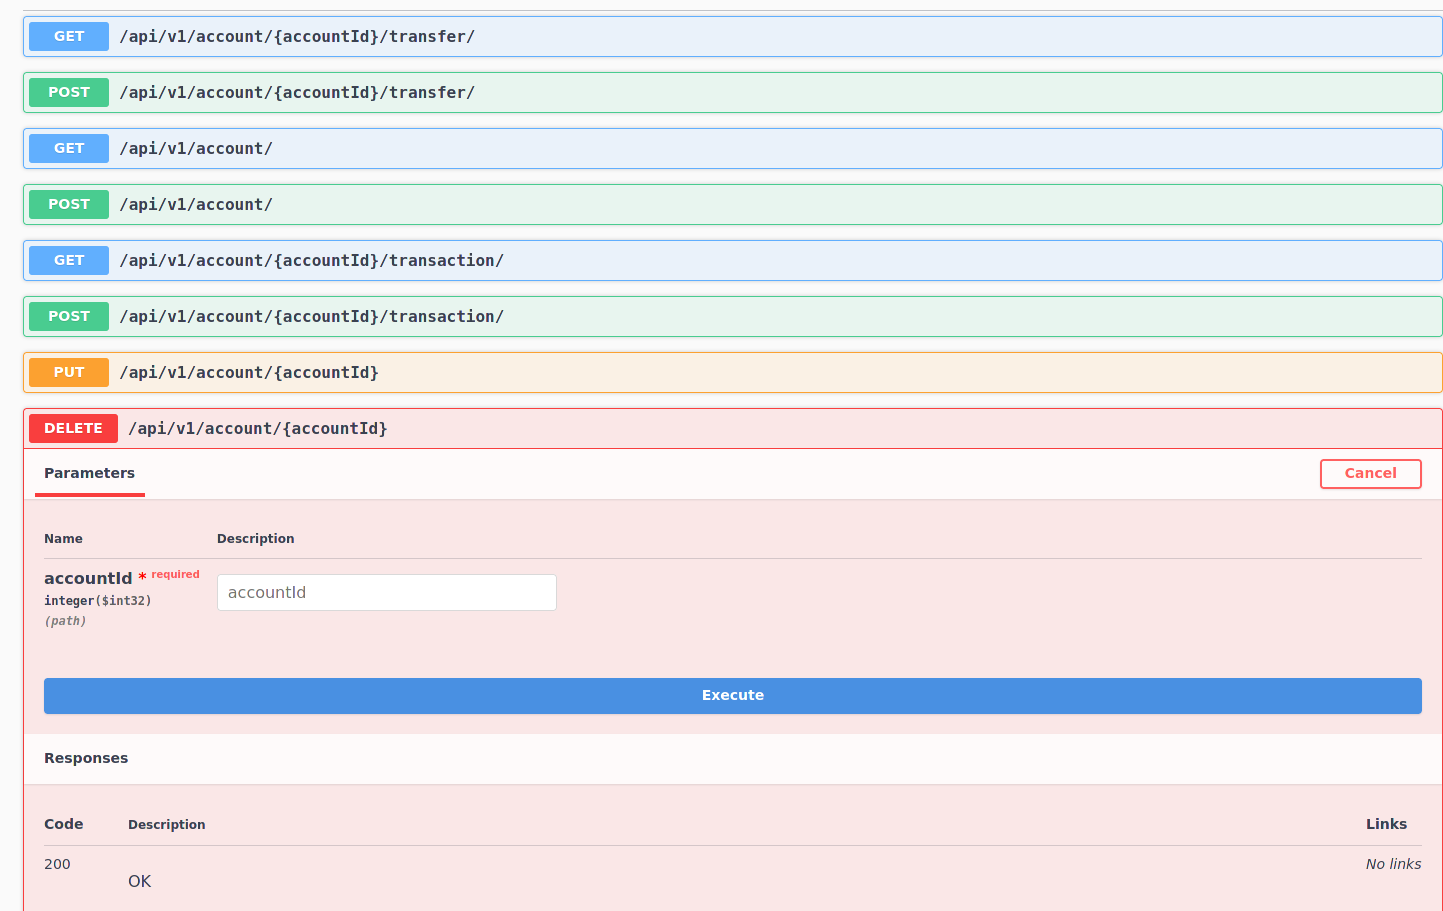
\includegraphics[scale=0.37]{screen-swagger.png}
	\caption{Dokumentacja API stworzona z użyciem Swagger UI}
	\label{fig:screen-category-add-form}
\end{figure}

\subsection{Schemat bazy danych}
Do przechowywania danych użyłem relacyjnej bazy danych PostgreSQL \citep{pgsql}. Schemat bazy wygenerowany z użyciem IDE IntelliJ IDEA \citep{idea} widoczny jest poniżej (Rys. \ref{fig:db-diagram}). Widzimy na nim tabele przechowujące dane kont, transakcji, transferów i kategorii. Miesięczne budżety przechowywane są w tabeli budgets. Każdy taki miesięczny budżet to kopia wszystkich kategorii wraz z przeznaczoną na nie kwotą i kwotą w ramach tej kategorii wydaną. Kategorie dla każdego budżetu przechowywane są w tabeli budgets\textunderscore categories.
\begin{figure}
	\centering
	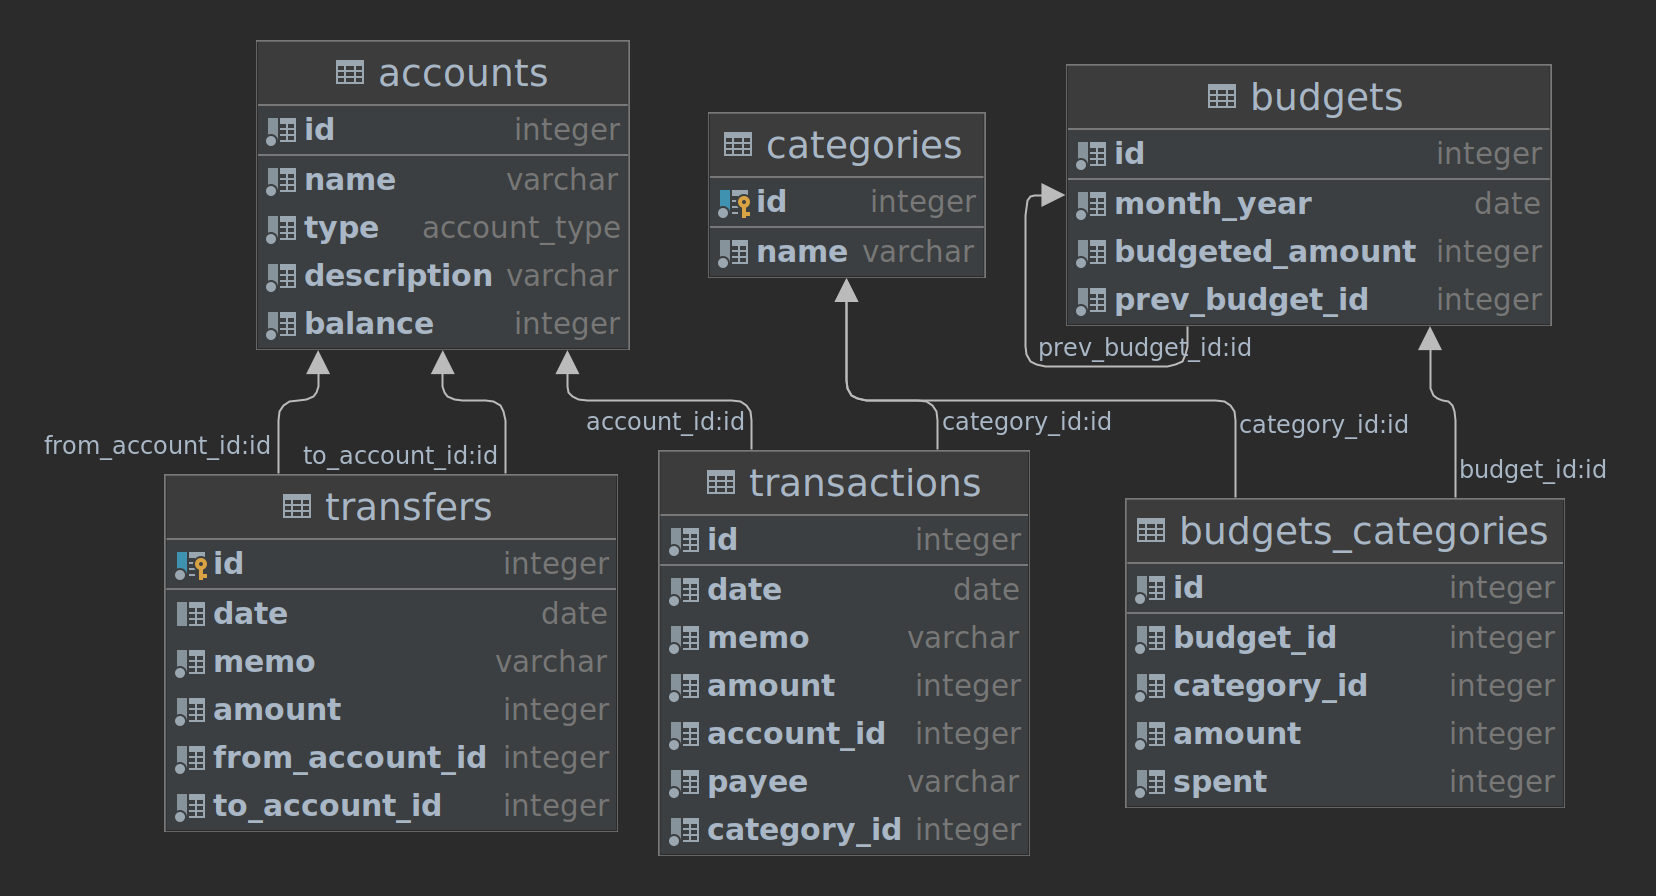
\includegraphics[scale=0.23]{db_diagram.png}
	\caption{Schemat bazy danych}
	\label{fig:db-diagram}
\end{figure}

Warstwa dostępu do danych używa frameworków Spring Data \citep{spring-data} oraz Hibernate ORM \citep{hibernate}. Hibernate używany jest w celu tłumaczenia danych z relacyjnego systemu typów wewnątrz bazy danych do obiektowego systemu w języku Java i używa wzorca projektowego Unit of Work \citep{uow}. Pozwala on oznaczać klasy jako tzw. encje, które odpowiadają tabelom w bazie danych. Hibernate automatycznie generuje zapytania w języku SQL na podstawie języka DSL o nazwie HQL lub na podstawie kodu w języku Java. Na bazie tego frameworka stworzony jest kolejny używany w tej warstwie, czyli Spring Data JPA, który używa wzorca Repository. \citep{repository}. Idzie on jeszcze o krok dalej niż Hibernate i dostarcza gotowe interfejsy, które implementują podstawowe metody dostępu do danych, czyli CRUD od create, retrieve, update i delete. Te rozwiązania wyręczają nas w tworzeniu prostych zapytań SQL, które wygenerują za programistę W moim rozwiązaniu używam takich wygenerowanych zapytań, ale też definiuję swoje tam, gdzie potrzeby aplikacji wykraczają poza opcje tych bibliotek.
\subsection{Inne technologie użyte w  części serwerowej}
\subsection*{MapStruct}
W aplikacji używam wzorca projektowego Data Transfer Object \citep{dto-pattern} (DTO), aby oddzielić dane udostępniane w API REST od reprezentacji danych w programie. Biblioteka MapStruct \citep{mapstruct} używana jest w aplikacji, aby zautomatyzować proces tworzenia obiektów DTO, który jest żmudny i powtarzalny dla każdej klasy. MapStruct automatycznie generuje kod tłumaczący obiekty modelu aplikacji na obiekty transferu danych.
\subsection*{Lombok}
Kod w języku Java uważany jest za zbyt rozwlekły w pewnych przypadkach. Programista musi pisać powtarzalny kod dla konstruktorów obiektów, metod dostępu i ustawiania danych (tzw. getters i setters) lub wzorca projektowego Builder \citep{builder-pattern}. Bibliotka Lombok stara się wyręczyć programistę w tych zadaniach poprzez automatyczną generację kodu. W mojej aplikacji używam przede wszystkim automatycznego tworzenia konstruktorów obiektów oraz metod tzw. getter i setter. Dzięki temu kod jest zwięzły i nie muszę zajmować się pisaniem takiego samego kodu dla różnych klas.
\subsection*{Hibernate Validator}
W mojej aplikacji używam także biblioteki Hibernate Validator \citep{hibernate-validator} do walidacji modelu danych, aby wszystkie wartości były poprawne. Pozwala ona zdefiniować walidację ograniczeń dla danych w aplikacji za pomocą adnotacji w języku Java. Biblioteka ta udostępnia zbiór gotowych reguł takich jak ograniczenia dla minimalnych i maksymalnych wartości danych liczbowych, ograniczenie wartości daty do dat przeszłych, ograniczenie długości napisów i wiele innych. Wybrałem tę bibliotekę, gdyż oferuje takie często używane ograniczenia dla danych, dzięki czemu nie muszę ich po raz kolejny implementować. Hibernate Validator automatycznie sprawdzi, czy dane są poprawne. Kod aplikacji nie jest wtedy zaśmiecany walidacją i skupia się na logice biznesowej.

\section{Część kliencka}
W odróżnieniu od części serwerowej, część kliencka została stworzona z użyciem języka JavaScript. Jej zadaniem jest komunikacja z częścią serwerową przy użyciu protokołu HTTP i prezentacja danych użytkownikowi. Została napisana przy użyciu biblioteki React \citep{react}, czyli popularnego rozwiązania do tworzenia interfejsu użytkownika.
\subsection{Biblioteka React}
React to biblioteka stworzona przez programistów Facebooka. Jest obecnie jedną z najchętniej wybieranych technologii do tworzenia interfejsów użytkownika \citep{react-popularity}, co przemawia nad jej wyborem z powodu mnogości dostępnych materiałów. Używanie tej technologii polega na podziale interfejsu na tak zwane komponenty. Są to podstawowe części tworzące interfejs, które są od siebie izolowane i łączone w większą całość oraz zarządzające swoim własnym stanem. Pozwala to tworzyć interaktywny interfejs strony, który zmienia się pod wpływem interakcji ze strony użytkownika bez potrzeby odświeżania całej strony. Efektywność tego rozwiązania jest polepszona dzięki użyciu wirtualnego DOM \citep{virtual-dom}. Wzorzec ten poprawia responsywność strony poprzez aktualizowanie tylko zmienionych elementów struktury DOM \citep{dom} zamiast wszystkich co jest tańszą operacją. Dzięki temu mogłem z łatwością stworzyć złożony i szybki interfejs myśląc o podstawowych elementach jakimi są komponenty. Niektóre z nich używane są w kilku miejscach dzięki czemu cały program składa się z mniejszej ilości kodu.

\subsection{Redux}
Wraz z rozwojem aplikacji interfejs stawał się coraz bardziej skomplikowany, a przy tym zarządzanie stanem komponentów stawało się coraz trudniejsze, gdyż ilość danych także rosła. Rozwiązaniem tego problemu jest użycie biblioteki Redux \citep{redux}. Używając tej technologii przechowujemy dane w jednym miejscu - obiekcie store. Komponenty interfejsu subskrybują zmiany w tym obiekcie i zmieniają się pod ich wpływem. Przepływ danych następuj więc w jedną stronę od obiektu store do interfejsu. Stan przechowywanych danych zmieniany jest z użyciem czystych funkcji nazywanych w tym wzorcu reducers:

\[ f(state, action) => newState \]

Takie funkcje nie mogą mieć efektów ubocznych ani zmieniać aktualnego stanu. Na podstawie danych wejściowych zwracają nowy stan powstały na bazie poprzedniego.
\begin{figure}
	\centering
	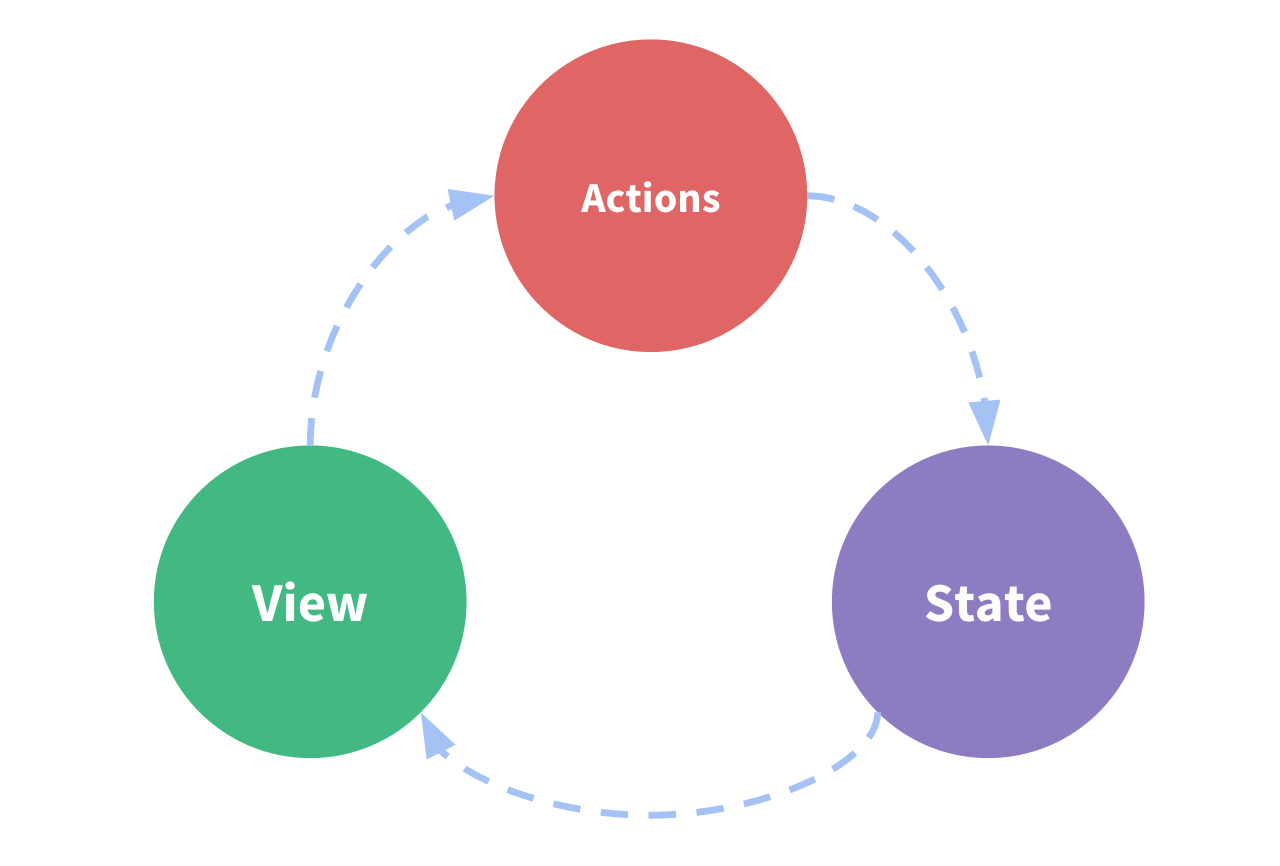
\includegraphics[scale=0.5]{redux-flow.png}
	\caption{Przepływ danych w architekturze używającej biblioteki Redux}
	\label{fig:redux-flow}
\end{figure}

Kod części klienckiej podzielony jest według funkcjonalności, których obsługa znajduję się w różnych podkatalogach. Obiekt store także jest podzielony między różne pliki obsługujące dane różnych rodzajów. Komponenty interfejsu użytkownika zlecają wykonywanie akcji obiektowi store oraz odczytują i aktualizują przechowywane w nim dane. Biblioteka Redux zajmuje się także komunikacją z częścią serwerową pobierając dane do obiektu store oraz wysyłając zmiany danych, gdy zmienia się ich stan po stronie klienckiej.

\subsection{Ant Design}
Aby ułatwić sobie tworzenie dobrze wyglądającego interfejsu użytkownika, użyłem biblioteki gotowych komponentów Ant Design \citep{ant-design}. Udostępnia ona spójne wizualnie elementy interfejsu użytkownika, które zostały stworzone z zachowaniem najważniejszych zasad dziedziny User Experience (UX). Jako, że elementy te są komponentami biblioteki React, połączenie ich z aplikacją jest niezwykle łatwe.
\begin{figure}
	\centering
	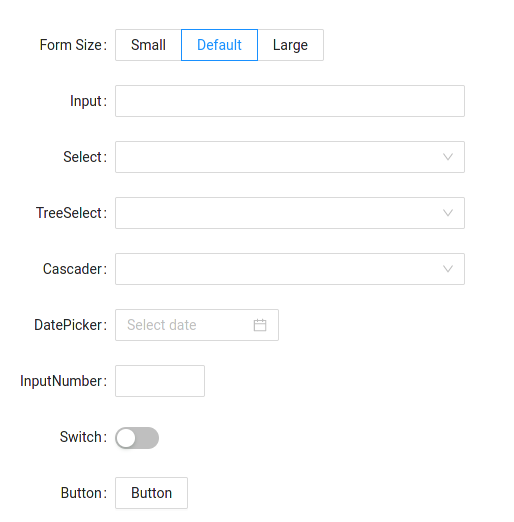
\includegraphics[scale=0.7]{screen-ant-design-form.png}
	\caption{Przykład gotowego komponentu z biblioteki Ant Design - formularz składający się z różnych komponentów do wprowadzania danych}
	\label{fig:ant-design-example}
\end{figure}

\subsection{Wykresy}
Do stworzenia wykresów używanych na podstronie dotyczącej statystyk użyłem gotowych bibliotek. Jedną z nich jest biblioteka Apex Charts \citep{apex-charts}, która udostępnia zbiór wielu dopracowanych wizualnie i interaktywnych wykresów dla różnych frameworków front-endowych, w tym używanego przeze mnie React. 
\begin{figure}
	\centering
	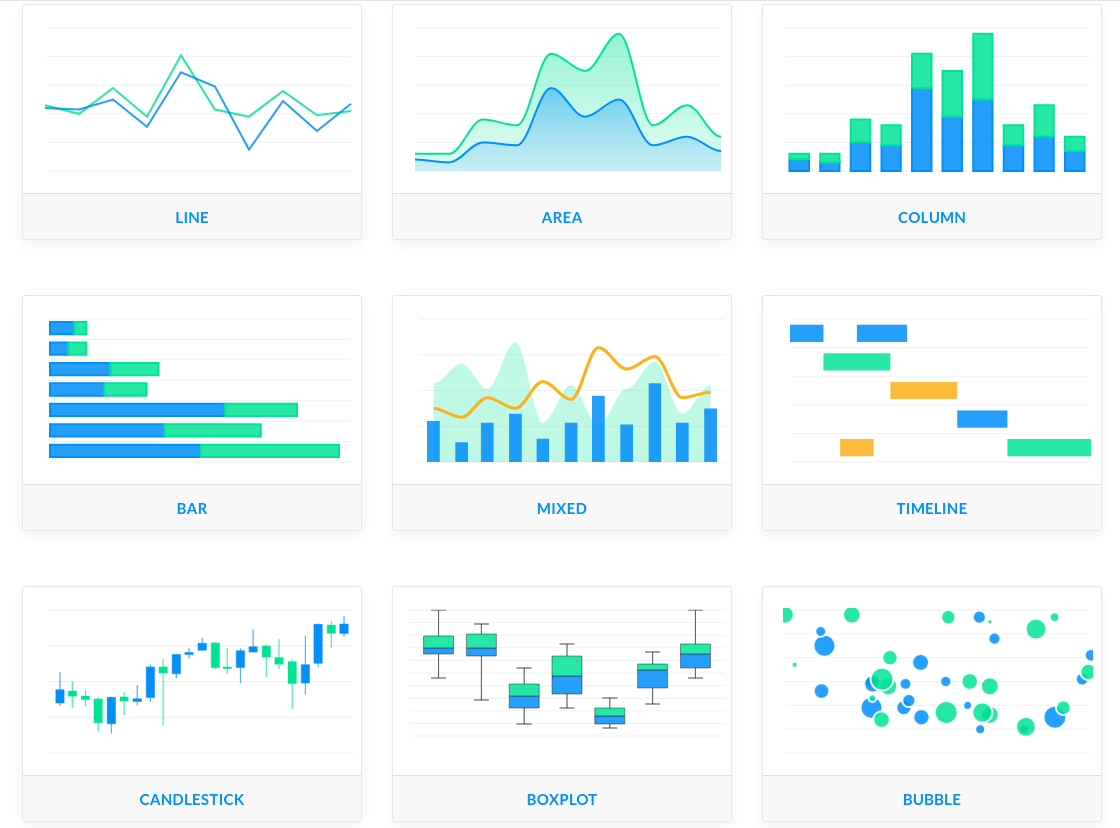
\includegraphics[scale=0.5]{screen-apex-demos.png}
	\caption{Różne rodzaje wykresów dostępne w bibliotece Apex Charts}
	\label{fig:apex-demos}
\end{figure}

Aby stworzyć wykres typu heatmap użyłem kolejnej biblioteki React Heat Map \citep{heatmap}, która stworzona została specjalnie do wyświetlania danych w postaci kalendarza, tzn. dla każdego dnia oddzielnie. 

\chapter{Podsumowanie}
\section{Możliwości dalszej rozbudowy}
Pisząc aplikację starałem się, aby była ona otwarta na dalsze usprawnienia. Poniżej przedstawiam kilka możliwych sposobów na ulepszenie aplikacji.
\subsection{Automatyczne dodawanie transakcji}
Dodawanie wszystkich transakcji i transferów ręcznie jest żmudne. Można więc to poprawić poprzez automatyczne pobieranie transakcji z kont bankowych użytkownika. Wymagałoby to dostępu do raportów z bankowości elektronicznej lub użycia API udostępnianego przez różne instytucje finansowe. Aplikacja mogłaby też posiadać funkcję odczytywania danych z paragonów, aby użytkownik nie musiał wpisywać ich ręcznie, a także pozwalałaby je zapisywać, aby były od razu dostępne w historii operacji.
\subsection{Konta użytkowników}
Obecnie aplikacja przeznaczona jest dla jednego konta co jest dużym ograniczeniem. Dodanie kont użytkowników, którzy prowadziliby oddzielnie dla siebie budżety byłoby więc dużym usprawnieniem aplikacji. Wymagałoby to dodania mechanizmu autoryzacji i uwierzytelniania oraz bezpiecznego przechowywania danych użytkowników. Po zaimplementowaniu takiej funkcjonalności można by było też udostępnić bezpiecznie aplikację przez Internet.
\subsection{Podział transakcji na kilka kategorii}
Niektóre transakcje stanowią pojedynczą operację finansową, ale składają się z transakcji w wielu kategoriach, np. w ramach jednej zapłaty za produkty w sklepie wydajemy pieniądze w różnych kategoriach. Dodanie opcji podziału transakcji na kilka kategorii usprawniłoby używanie aplikacji, gdyż historia operacji zapisanych w aplikacji lepiej odzwierciedlałaby rzeczywiste operacje.
\section{Wnioski końcowe}
Pomysł na aplikację wziął się także z moich prywatnych potrzeb, gdyż nie chciałem przechowywać informacji o budżecie na zewnętrznych serwerach. W ramach tej pracy udało mi się stworzyć aplikację z podstawowymi funkcjonalnościami, które są wystarczające, aby rozpocząć zarządzanie budżetem osobistym. Tworząc ten program miałem okazję poznać nowoczesne technologie z różnych dziedzin - zarówno używane po stronie serwera, jak i przeglądarki internetowej.
%%%%% BIBLIOGRAFIA

\bibliographystyle{unsrt}
\bibliography{bibliography}

\end{document}
